\documentclass[10pt,a4paper]{article}
\usepackage{researchsketch} % See researchsketch.sty %
\usepackage{enumitem}
\usepackage{algorithm}
\usepackage{algpseudocode}
\usepackage{hyperref}
\setenumerate[1]{itemsep=0pt, partopsep=0pt,topsep=5pt}
\setitemize[1]{itemsep=0pt, partopsep=0pt,topsep=5pt}
\author{1155189917}
\title{Draft}
\pagestyle{fancy}
\renewcommand{\headrulewidth}{0pt}
\fancyhf{}
\rfoot{Page \thepage}
\date{\today}
\begin{document}
\noindent On Robustness of Quantized Neural Network Optimizations (Quantization-Aware Training)\hfill Draft\\
WONG, Hok Fong\hfill UG Summer Research Internship\hfill Last Updated: 31 Jul, 2024\\
\phantom{}\hrulefill

\section{Background}

\subsection{Towards the Time- and Energy-Efficient, Optimal Neural Network Design}

\subsection{State-of-the-Art Fine-tuning Methods in Quantization-Aware Training Procedures}

\subsubsection{BinaryConnect}

\subsubsection{Straight-Through Estimators}

\subsection{Formalization of the Optimization Problem and Inherent Difficulty}

\section{Preliminaries}


In this section, we will consider the following optimization problem:
\begin{equation}\label{P}\tag{P} \min\limits_{x\in C} \ell(x), \text{where } C:=\{x\in \mathbb{R}^n \bigm| g(x)\geq 0\}\end{equation}
with the objective function $f:\mathbb{R}^n\rightarrow \mathbb{R}$, and constraints described by the function $g: \mathbb{R}^n \rightarrow \mathbb{R}^d$.



\subsection{Muehlebach-Jordan's Work on Local Approximation of the Constraint Set} \phantom{}

\assumption{\label{ass1}
    The functions $\ell$, $g$ are continuously differentiable and have an $L$-Lipschitz continuous gradient. Additionally, $\ell$ is lower-bounded.
}

\assumption{\label{ass2}
    The Mangasarian-Fromovitz constraint qualification (MFCQ) is satisfied for all $x\in \mathbb{R}^n$, i.e. $\forall x\in \mathbb{R}^d$, $\exists w\in \mathbb{R}^n$ s.t. $\nabla g_i(x)w>0$ for all $i\in I(x)$, where $I(x)=\{i\in \mathbb{Z}\bigm| g_i(x)\leq 0\}$.
}

\begin{algorithm}
    \caption{Muehlebach-Jordan's First-Order Gradient Flow Algorithm}\label{alg:cap}
    \begin{algorithmic}[1]
        \State Start with an initial dual guess $x_0\in\mathbb{R}^d$
        \For {$k=0, 1, \ldots$}
        \State Let $-R_k\in\partial \psi_{V_\alpha(x_k)}((x_{k+1}-x_k)/T)$
        \State $x^{(k+1)}\gets x^{(k)}-T\nabla f(x_k)+TR_k$
        \EndFor
    \end{algorithmic}
\end{algorithm}

Additionally, Muehlebach and Jordan (2022) have shown the equivalence between $-\nabla f(x_k)+R_k$ and \begin{equation}\label{speed}\argminnl_{v\in V_\alpha(x)}(1/2)\lVert v+\nabla f(x)\rVert^2\end{equation} due to Assumption \hyperref[ass2]{2}. We emphasize this formulation for its characterization of the behavior of the above algorithm (and the algorithms developed in this paper).

\subsection{Constructing a Constrained Quantization Function} \phantom{}

Leconte et al.'s (2023) approach to the optimization problem relaxes the quantization constraints to a set of ``smoothed'' interval constraints. They first create a continuous function that quantifies "how far away" a parameter is from its quantization levels.

\definition{
    Let $\eps\in[0,1]$, $w^i \in \mathcal{Q}^i, i\in \{1, 2, \ldots, d\}$, i.e. each $w^i$ coordinate-wisely takes value from its own set of quantization levels $\mathcal{Q}^i=\{q_1^i, q_2^i, \ldots, q_{K^i}^i\}$. We define the piecewise function $$\psi_\eps^i(w^i):=\begin{cases}\epsilon-(q^i_{1}-w^i)^2,& w^i < q^i_{1},\\\eps-(w^i-q^i_{j-1})^2(w^i-q^i_j)^2,& q^i_{j-1}\leq w^i < q^i_{j}, j=2,\ldots, K,\\\eps-(w^i-q^i_{K})^2,& w^i \geq q^i_{K^i},\end{cases}$$ for all $w^i\in\mathbb{R}$.
}

\assumption{
    The stepsizes $(\gamma_k)_{k\geq 0}$ are positive, $\sum_{k=0}^\infty \gamma_k=\infty$ and $\lim_{k\to\infty} \gamma_k=0$.
}

\assumption{
    $\sum_{k=0}^\infty \gamma^2_k<\infty$.
}

We can simplify the tangent cone and the normal cone for any $x\in C$ as follows, due to the Mangasarian-Fromovitz constraint qualification of $g$: $$T_C(x)=\{x\bigm|\nabla g_i(x)^{\top} x\geq 0, \forall i \in I_x\}, N_C(x)=\left\{\lambda\in \mathbb{R}^d_{+}\middle|-\sum_{i\in I(x)} \lambda_i \nabla g_i(x)\right\}.$$

\definition{
    Further define the set $V_{\eps, \alpha}(x):=\{v\in \mathbb{R}^n\bigm|\nabla g_i(x)^{\top}v+\alpha g_i(x)\geq 0, \forall i \in I_x\}$, where $\alpha>0$.
}

\noindent\textbf{Condition A.} $V_\alpha(w)$ is empty if and only if there is $1\leq i\leq d$ such that $w^i=(q^i_{Q^i(w^i)}+q^i_{Q^i(w^i)+1})/2$\label{cond1}.

Indeed. For the case where $x\in C$, $V_\alpha(x)$ is nothing but $T_C(x)$. Otherwise, consider any $g_i(x)<0$ for some $i$, by MFCQ there exists $u$ such that $\forall i\in I_\eps(x), \nabla g_i(x)^{\top} u> 0$ and therefore by scaling we have $\nabla g_i(x)^\top v\geq -\alpha g_i(x)\geq 0$.

We consider following formulation for the update direction again, and observe that under the current settings, $$v_{k}=\argminnl_{v\in V_{\eps,\alpha}(w_k)}(1/2)\lVert v+\widehat{\nabla\ell}(w_k)\rVert^2$$ admits an explicit solution $$[s_{\eps,\alpha}(\widehat{\nabla\ell}(w_k), w_k)]^i=\begin{cases}-\widehat{\nabla\ell}(w_k^i),& \text{if }\psi_\eps(w^i)>0\text{ or } -\psi'_\eps(w^i)\widehat{\nabla\ell}(w_k^i)\geq -\alpha\psi_\eps(w^i)>0,\\\text{clip}(-\alpha\psi_\eps(w^i)/\psi'_\eps(w^i), M_{\eps}),& \text{otherwise},\end{cases}$$for $w$ such that $w^i\neq (q^i_{Q^i(w^i)}+q^i_{Q^i(w^i)+1})/2$, where $Q^i(w^i)$ is the unique index satisfying $q^i_{Q^i(w^i)}\leq w^i<q^i_{Q^i(w^i)+1}$.

\begin{algorithm}
    \caption{The \texttt{ASkewSGD} Algorithm}\label{alg:cap}
    \begin{algorithmic}[1]
        \State Select a sequence $(\gamma_k)$ of step sizes, and size of the mini-batch $N_b\leq N$.
        \State Start with an initial dual guess $x_0\in \mathbb{R}^d$
        \For {$k=0, 1, \ldots$}
        \State Sample a mini-batch of $N_b$ observations $\{j_1, j_2, \ldots, j_{N_b}\}$ in $\{1,2, \ldots, N\}$
        \State Compute the stochastic gradient $\widehat{\nabla}\ell(w_k)=1/N_b \sum_{i=1}^{N_b} \nabla\ell(w_k; \xi_{j_i})$
        \State Compute the update direction $v_k=s_{\eps, \alpha}(\widehat{\nabla\ell}(w_k), w_k)$
        \State $x^{(k+1)}\gets x^{(k)}-\gamma_k v_k$
        \EndFor
    \end{algorithmic}
\end{algorithm}

\subsection{Unconstrained Minimax Optimization by Lagrangian Multipliers} \phantom{}

\section{Convergence Proof}

In this section, we follow the work of Muehlebach and Jordan's (2022) to analyze the convergence of the deterministic version of \texttt{ASkewSGD} under our new construction for the constraint set $C_{\eps}$.

The novelty of our new setup has successfully extended the constructions by Leconte et al. (2023) toward better properties including piecewise convexity, and constraints separation for every quantization level etc. This fact is helpful if we need to characterize the smoothness\footnote{Note that in the context of optimization, smoothness controls the changes in gradients.} of the Lagrangian dual of (\ref{P})

\definition{
    We define the piecewise function $$\hat{\phi}^i(w^i):=\begin{cases}(q^i_{1}-w^i),& w^i < q^i_{1},\\(q^i_{j-1}-w^i)(w^i-q^i_j),& q^i_{j-1}\leq w^i < q^i_{j}, j=2,\ldots, K,\\w^i-q^i_{K},& w^i \geq q^i_{K^i},\end{cases}$$ for all $w^i\in\mathbb{R}$.
}

Observing the convexity of $\psi$, it would be natural to think about whether we treat every convex piece independently.

\definition{
    A function $F: \mathbb{R}^n \mapsto \mathbb{R}$ is called a piecewise convex function if it can be decomposed into: $$F(x) = \min\{f_1(x), f_2(x), \ldots, f_m(x)\},$$ where $f_j: \mathbb{R}^n \mapsto \mathbb{R}$ are convex functions for all $j \in [M]$.
}
\lemma{
    Let $\eps\in [0,1]$, $\hat{\psi}^i(w^i):=\eps-\hat{\phi}^i(w^i)$ is a piecewise convex function.
}
\begin{proof}
    That is, to prove that $\hat{\psi}$ can be decomposed into concave functions $f_1, \ldots, f_m$ where $F(x)=\max(f_1(x), f_2(x), \ldots, f_m(x))$.

    \begin{center}
        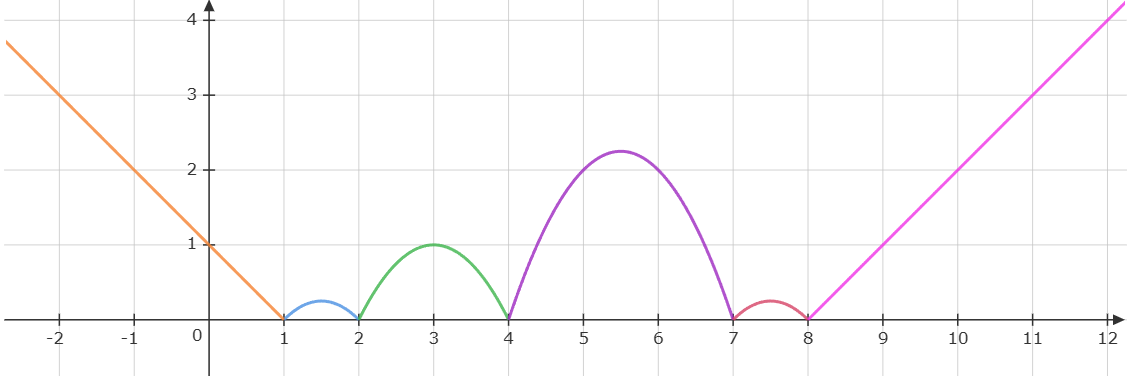
\includegraphics[width=0.5\linewidth]{psi.png}
    \end{center}

    Select $m=K+1$ such that the $f_i$'s $(i=1, \ldots, K+1)$ corresponds to the analytic continuation of every piece of the piecewise function:

    $$\begin{cases}f^i_1(w^i):=(q^i_{1}-w^i),\\f^i_j(w^i):=(q^i_{j-1}-w^i)(w^i-q^i_{j}), j=2,\ldots, K^i,\\f^i_{K^i+1}(w^i):=w^i-q^i_{K^i}.\end{cases}$$

    The proof is pictorially shown by the plot above. Observe that any $f^i_j>0$ implies $f^i_k<0$ for any $j\neq k$, this is guaranteed by the choice of $f_i$s (being linear or quadratic functions).
\end{proof}

\corollary{
The constraint on the $i$-th parameter $w^i$ described by $g_i:=\{w^i: \hat{\psi}^i(w^i)\geq 0\}$ can be replaced by $g'_i=(f^i_1, \ldots, f^i_{K^1})\succeq0$.
}

This corollary is direct from the definition of piecewise convex function. For the purpose of simplicity, we first adopt the original constraint functions described by $\phi^i$ instead of $f^i_j$. We will explicitly state when we apply the replacement.

\theorem{\label{convthm2}    Under Assumption 1 and 3 and $0<\eps\leq \inf_{1\leq i\leq d}\inf_{1\leq j\leq K^i} \abs{c_j^i - c_{j+1}^i}^2/4, \alpha\leq L$, where $\{c_j^i\}$ are the quantization levels. Then, $\ell(w_k)$ converges and $\lim_{k\to\infty} d(w_k, \mathcal{Z}_\eps)=0$ almost surely.
}

Again, we have followed the journey of Muehlebach and Jordan's (2022) work. Their convergence proof hinges heavily on the properties that:

\begin{itemize}
    \item Once $w_k$ has fallen into a convex region $C$, the multiplier $\lambda_k$ is feasible for the dual (\ref{speed}) at time $k+1$.
    \item The function $\mathcal{L}(x_k,\lambda_k)-\lVert\nabla_x\mathcal{L}(x_k,\lambda_k)\rVert^2/2\alpha$ increases from $x_k$ to $x_{k+1}$ (for a fixed $\lambda_k$) due to the smoothness of $\ell$.
\end{itemize}

The proof of Theorem \hyperref[convthm2]{\thetheoremcnt} is done by several smaller lemmata. First, we bounding the step size such that the iterates fall into a convex region. Then, we show that the corresponding dual of (\ref{speed}) $d(x_k)$ is monotonically increasing and bounded above by $f^*$. Finally, we expand $d(x_{k+1})$ as a telescoping sum, and it immediately follows that $v_k$ converges to zero for large $k$.

\lemma{
    Strong duality holds for (\ref{speed}) for every $x\in\mathbb{R}^n$ when $V_{\alpha,\eps}$ is non-empty (See \hyperref[cond1]{Condition A}). For $\alpha\geq 0$, the dual can be rewritten as \begin{equation}\label{speeddual}\max\limits_{\lambda\succeq 0} -\frac{1}{2}\lVert\lambda^\top\nabla g(x)-f(x)\rVert^2-\alpha\lambda^\top g(x)\end{equation}
}
\begin{proof}
    Let $D_x:\{\lambda\in \mathbb{R}^n: \lambda_i=0\text{ if }i\notin I(x)\}$. For clarity, we reformulate the primal problem in Lagrangian:

    \begin{equation} \min\limits_{v\in\mathbb{R}^n} \max\limits_{\lambda\in D_x} \frac{1}{2} \lVert v+ \nabla f(x)\rVert^2-\lambda^{\top}(\nabla g(x)^{\top}v+\alpha g(x)).\end{equation}

    Then, the corresponding dual is as follows:

    \begin{equation} \max\limits_{\lambda\in D_x} \min\limits_{v\in\mathbb{R}^n}  \frac{1}{2} \lVert v+ \nabla f(x)\rVert^2-\lambda^{\top}(\nabla g(x)^{\top}v+\alpha g(x)),\end{equation}

    which then resolves into (\ref{speeddual}) by picking $v^*=\lambda^{\top}\nabla g(x)-\nabla f(x)$ and the addition of the constant term $-(1/2)\lVert\nabla f(x)\rVert^2$.

    We show that Slater's condition holds for $V_{\eps, \alpha}$, i.e. there exists a $v\in \mathbb{R}^n$ such that $\nabla g_i(x)^{\top} v+\alpha g_i(x)>0$ for all $i\in I_\eps(x)$.

    Let $\bar{v}\in \mathbb{R}^n$ satisfy $\nabla g_i(x)\bar{v}+\alpha g_i(x) = 0, \forall i \in I_\eps(x)$. By MFCQ, there exists a $w\in \mathbb{R}^n$ such that $\nabla g_i(x)w>0, \forall i\in I_\eps(X)$. Picking $v=\bar{v}+\xi w$ for some $\xi>0$ satisfies the required condition.

    By the fact that (\ref{speed}) is convex,
\end{proof}











\newpage
\noindent\textbf{Fact.} The MFCQ condition is automatically satisfied for $x\in C_\eps$ by construction.



Tangent cones have a natural role in the theory of flow-invariant sets and gradient inclusions.

\definition{
    The Clarke's tangent cone of $C$ contains all $\delta x\in T_C(x)$ if there exists two sequences $x_j\rightarrow x, x_j \in C, t_j\downarrow 0$ such that $(x_j-x)/t_j\rightarrow \delta x$. The normal cone is defined as follows: $N_C(x)=\{\lambda\in \mathbb{R}^n\bigm| \lambda^{\top}\delta x\leq 0, \forall \delta x\in T_C(x)\}$.
}

\lemma{
    Suppose that $x\in C$, then every $\delta x\in T_C(x)$ satisfies $\nabla g_i(x)\delta x\geq 0, \forall i\in I_x$. The converse also holds.
}

\begin{proof}
    $(\Rightarrow):$ $\delta x\in T_C(x)$ implies that there exists two sequences $\{x_j\}\rightarrow x, \{x_j\}\subset C, t_j\downarrow 0$ for all $j\in \mathbb{N}$ and $$\frac{x_j-x}{t_j}\rightarrow \delta x,$$ which implies that $$\frac{g(x_j)-g(x)}{x_j-x}\cdot\frac{x_j-x}{t_j}\geq 0.$$ This is because $x_j\in C$ implies that $g_i(x_j)\geq 0$ and $g_i(x)\leq 0$ for all $i\in I(x)$.

    $(\Leftarrow):$ Adapted from R. Herzog, 2023, a simplified version. Let $\delta x$ satisfy $\nabla g_i(x)\delta x\geq 0, \forall i\in I_x$, also let $\delta y$ be given by MFCQ such that $\nabla g_i(w)\delta y>0, \forall i \in I(x)$. Put $\ell(t):=\delta x+ t\cdot\delta y$. Then for all $t>0$, we have $\nabla g_i(x) \ell(t)>0, \forall i\in I(x)$, implying that $\ell(t)$ are all feasible MFCQ vectors.

    Now, we claim that $\ell(t)\in T_C(x)$ for all $t\in \mathbb{R}_{++}$. Let $\gamma(t):=x+t\ell(t)$, $t\in(-\eps, \eps)$, for an infinitestimally small $\epsilon$, given by the continuity of $g$. Then, $y(t)\in C$ for every $t\in [0, \epsilon)$ and $\gamma(0)=x, \gamma'(0)=\ell(t)$. For an arbitrary sequence $\{t_j\}\downarrow0$ and $x_k = \gamma(t_j)\rightarrow x$ we have $$\ell(t)=\gamma'(0)=\lim_{j\to\infty} \frac{\gamma(t_j)-\gamma(0)}{t_j-0}=\lim_{j\to\infty}\frac{x_j-x}{t_j}\in T_C(x).$$

    Since $T_C(x)$ is closed, $\delta x=\lim_{t\to0}\ell(t)\in T(x)$.
\end{proof}

Now, we can simplify the tangent cone and the normal cone for any $x\in C$ as follows, due to the Mangasarian-Fromovitz constraint qualification: $$T_C(x)=\{x\bigm|\nabla g_i(x)^{\top} x\geq 0, \forall i \in I_x\}, N_C(x)=\left\{\lambda\in \mathbb{R}^d_{+}\middle|-\sum_{i\in I(x)} \lambda_i \nabla g_i(x)\right\}.$$

\definition{
    Further define the set $V_\alpha(x):=\{v\in \mathbb{R}^n\bigm|\nabla g_i(x)^{\top}v+\alpha g_i(x)\geq 0, \forall i \in I_x\}$, where $\alpha>0$. $V_\alpha(x)$ is guaranteed to be non-empty for any $x$.
}

Indeed. For the case where $x\in C$, $V_\alpha(x)$ is nothing but $T_C(x)$. Otherwise, consider any $g_i(x)<0$, by MFCQ there exists $u$ such that $\nabla g_i(x)^{\top} u> 0$ and therefore by scaling we have $\nabla g_i(x)^\top v\geq -\alpha g_i(x)\geq 0$.

\definition{
    The indicator function for a set $C$ is defined as:

    $$\psi_C(x)=\begin{cases}
            0,      & x\in C,           \\
            \infty, & \text{otherwise}.
        \end{cases}$$
}
\theorem{
Let $x:[0, \infty)\rightarrow \mathbb{R}^n$ be an absolutely continuous trajectory with a piecewise continuous derivative. Then, for any $x(0)\in C$, the following are equivalent:

$$\begin{aligned}
         & \dot{x}(t):=-\nabla f(x(t))+R(t), -R(t)\in N_C(x(t)),                                           &  & \forall t\in [0, \infty) \text{ almost everywhere}, \\
         & \dot{x}(t)^+:=-\nabla f(x(t))+R(t), -R(t)\in \partial\psi_{V_\alpha(x(t))}(\dot{x}(t)^+),       &  & \forall t\in[0, \infty),                            \\
         & \dot{x}(t)^+:=-\argmin_{v\in V_{\alpha}(x(t))}{\frac{1}{2}\abs{v+\nabla f(x(t))}^2}, \phantom{} &  & \forall t\in[0,\infty).
    \end{aligned}$$
}

\lemma{Using the \texttt{ASkewSGD} algorithm with step sizes $\{\gamma_k\}$ of $\sum_{i=1}^\infty \gamma_i=\infty$, $\sum_{i=1}^\infty \gamma_i^2<\infty$, the iterate $\{w_k\}$ is guaranteed to converge and $\lim_{k\to\inf} d(w_k,C_\epsilon)=0$.}

\begin{proof}
    See Leconte et al., 2023, Appendix A.3.
\end{proof}

\lemma{Let $k_0=\sup_{1\leq i\leq d,1\leq j\leq K_i}\sup\{k:\gamma_kM\geq\max(c_- - \frac{c_j^i+c_{j+1}^i}{2},-c_+ + \frac{c_j^i+c_{j+1}^i}{2})\}$. Since $w$ must }



\newpage
% \section{Derivation of Distance between $w$ and $C_\varepsilon$}

\newpage
\section{Lagrange Duality}
\noindent The problem $\mathcal{P}$ of $$\min\limits_{x\in C} f(x), C=\{x\in \mathbb{R}^n\bigm| g(x)\leq 0\}$$ is equivalent to the primal problem $$\inf\limits_{x\in \mathbb{R}^n}\sup\limits_{\lambda\succeq 0} f(x)+\sum\limits_{i=1}^d \lambda_i g_i(x).$$ We consider the dual problem $$\sup\limits_{\lambda\succeq 0}\inf\limits_{x\in \mathbb{R}^n} f(x)+\sum\limits_{i=1}^d \lambda_i g_i(x).$$

\theorem{
    Suppose that $x^{*}$ is a local minimizer of $\mathcal{P}$ which satisfies the MFCQ. Then there exist Lagrange multipliers $\lambda^*$ (not necessary unique) such that the KKT conditions are satisfied. The set of Lagrange multipliers $\Lambda(x^*)$ is compact.
}

Therefore, the KKT points can be captured by the following set: $$\mathcal{Z}_\eps=\{w\in C_\eps: 0\in -\nabla \ell(w)+N_{C_\eps}(w)\}$$

\theorem{
    If $f: \mathbb{R}^d \mapsto \mathbb{R}$ is twice continuously differentiable and satisfies the strict saddle property, then gradient descent with a random initialization and sufficiently small constant step size converges to a local minimizer or negative infinity almost surely. Call $x$ a critical point of $f$ if $\nabla f(x) = 0$, and say that $f$ satisfies the strict saddle property if each critical point $x$ of $f$ is either a local minimizer, or a “strict saddle”, i.e, $\nabla^2 f(x)$ has at least one strictly negative eigenvalue.(J. D. Lee, in PMLT, 2016)
}

% Define the function $f^i_j(w) = -\varepsilon + \psi^i_j(w)$ for $j=1,2,\ldots, K+1$, and $i$ stands for the $i$-th parameter of the model.

\begin{algorithm}
    \caption{Dual gradient ascent method (convex constraints)}\label{alg:cap}
    \begin{algorithmic}[1]

        \State Start with an initial dual guess $\lambda(0) \geq 0$.
        \For {$k=1, 2, \ldots$}
        \State $x^{(k)}\in \argmin\limits_{x} \ell(x)+(\lambda^{(k-1)})^{\top}g(x)$
        \State $\lambda^{(k)}=\max\{\lambda^{(k-1)}+\gamma_kg(x^{k}), 0\}$
        \EndFor
    \end{algorithmic}
\end{algorithm}

\assumption{
    The objective function $f$ is convex and continuously differentiable.
}

How we can find $x^*$ efficiently, as $\nabla \ell$ is implicit? % Pointed out that, it may be difficult to evaluate the dual (requires unconstrained minimization of Lagrangian). We can consider coordinate-wise descent but 

The problem is that $f(x)-\mathbf{\lambda}g$ is a combination of a convex and a concave function (where $g$ is convex and $g\geq 0$ is required).

\url{https://proceedings.neurips.cc/paper_files/paper/2023/file/a961dea42c23c3c0d01b79918701fb6e-Paper-Conference.pdf}

% \theorem{
%      Given convex, differentiable $f: \mathbb{R}^n \to \mathbb{R}$, if we are at a point $x^*$ such that $f(x^*)$ is minimized along each coordinate axis, then $x^*$ is a global minimizer, i.e. $f(x+\delta e_i)\geq f(x)$ for all $\delta, i$ leads to $f(x)=\min_z f(z)$.
% }


% Now we consider the subroutine of finding $x^{(k)}$ by the coordinate descent algorithm.

% Even though we have assumed convexity of the loss function $\ell$, the new algorithm is novel in the sense that:

% \begin{itemize}
%      \item New edits to the constraint function $\psi$ with piecewise convex properties.
%      \item We can precisely control the error bound of our weights by $\varepsilon$.
%      \item The annealing step is unnecessary - thus lowering the time complexity.
%      \item The function can be non-smooth, as long as convexity is guaranteed (Sub-gradient methods, and see Nesterov, 2012).
% \end{itemize}

% We also notice some limitations of our proposed method:

% \begin{itemize}
%      \item The algorithm cannot be extended to equality constraints due to the simultaneous minimization of multiple quantization constants.
%      \item The algorithm's complexity is determined by the quantization levels, with small tolerance of interval size.
% \end{itemize}


% \newpage
% \section{Discussions}

% \subsection{More ideas}
% Under the assumption of non-summable and square-summable step sizes, $\lim\sup_{k\to\infty} d(w_k, C_\epsilon)=0$ almost surely. Given that the current piece $C_\epsilon$ is convex, disconnected, can we guarantee that $d(w_k, \mathcal{Z}_{\epsilon})$ converges almost surely? Note that the direction picked by speed never guide $w$ to leave the feasible set if any constraint is already violated.  (Will continue to read Boob, 2019. \textit{arXiv}: \url{https://arxiv.org/pdf/1908.02734})

% First, we want to know if the algorithm escapes from saddle points (so not just stationary points but minimizers). (Stochastic case follows from \url{https://sites.math.washington.edu/~ddrusv/aiming_deep.pdf} and \url{https://hal.science/hal-03442137/file/tame.pdf}, step sizes \url{https://hal.science/hal-02564349/file/clarke.pdf})

% Second, yet another Gradient Flow inspection. (\url{https://openreview.net/pdf?id=xuw7R0hP7G})

% Third, experiment on C1-smooth and non C2-smooth functions (don't really know if they are even usable). Example: finding out the cases when the algorithm fails to converge?

% Fourth, another algorithm for non-convex optimization. (\url{https://arxiv.org/pdf/1908.02734})

% \subsection{A survey of quantization methods}

% \subsection{Updates on the numerical experiment}

% \subsection{Incoming Events}

\end{document}
